\documentclass{vgtc}

\ifpdf%                                % if we use pdflatex
  \pdfoutput=1\relax                   % create PDFs from pdfLaTeX
  \pdfcompresslevel=9                  % PDF Compression
  \pdfoptionpdfminorversion=7          % create PDF 1.7
  \ExecuteOptions{pdftex}
  \usepackage{graphicx}                % allow us to embed graphics files
  \DeclareGraphicsExtensions{.pdf,.png,.jpg,.jpeg} % for pdflatex we expect .pdf, .png, or .jpg files
\else%                                 % else we use pure latex
  \ExecuteOptions{dvips}
  \usepackage{graphicx}                % allow us to embed graphics files
  \DeclareGraphicsExtensions{.eps}     % for pure latex we expect eps files
\fi%

\graphicspath{{figures/}{pictures/}{images/}{./}} % where to search for the images

\usepackage{microtype}                 % use micro-typography (slightly more compact, better to read)
\PassOptionsToPackage{warn}{textcomp}  % to address font issues with \textrightarrow
\usepackage{textcomp}                  % use better special symbols
\usepackage{mathptmx}                  % use matching math font
\usepackage{times}                     % we use Times as the main font
\renewcommand*\ttdefault{txtt}         % a nicer typewriter font
\usepackage{cite}                      % needed to automatically sort the references
\usepackage{tabu}                      % only used for the table example
\usepackage{booktabs}                  % only used for the table example
\usepackage{listings}
\usepackage{xcolor}  % for custom colors

\definecolor{codegreen}{rgb}{0,0.6,0}
\definecolor{codegray}{rgb}{0.5,0.5,0.5}
\definecolor{codepurple}{rgb}{0.58,0,0.82}
\definecolor{backcolour}{rgb}{0.95,0.95,0.92}

\lstdefinestyle{mystyle}{
  backgroundcolor=\color{backcolour},   
  commentstyle=\color{codegreen},
  keywordstyle=\color{magenta},
  numberstyle=\tiny\color{codegray},
  stringstyle=\color{codepurple},
  basicstyle=\ttfamily\footnotesize,
  breakatwhitespace=false,         
  breaklines=true,                 
  captionpos=b,                    
  keepspaces=true,                 
  numbers=left,                    
  numbersep=5pt,                  
  showspaces=false,                
  showstringspaces=false,
  showtabs=false,                  
  tabsize=2
}

\lstset{style=mystyle}

%% If you are submitting a paper to a conference for review with a double
%% blind reviewing process, please replace the value ``0'' below with your
%% OnlineID. Otherwise, you may safely leave it at ``0''.
\onlineid{0}

%% declare the category of your paper, only shown in review mode
\vgtccategory{Research}

\title{Cauldron Chaos}

\author{Christoph Daxerer\thanks{e-mail: christoph.daxerer@chello.at}}
\affiliation{\scriptsize Software Engineering ba. VZ FH-Oberösterreich Hagenberg}

%% A teaser figure can be included as follows, but is not recommended since
%% the space is now taken up by a full width abstract.
%\teaser{
%  \includegraphics[width=1.5in]{sample.eps}
%  \caption{Lookit! Lookit!}
%}

%% Abstract section.
\abstract{
  For the V1\_VIREIL Virtual Reality course this paper describes the 
  design and impelemntation of a potion mixing game for the HTC Vive.
} % end of abstract


%%%%%%%%%%%%%%%%%%%%%%%%%%%%%%%%%%%%%%%%%%%%%%%%%%%%%%%%%%%%%%%%
%%%%%%%%%%%%%%%%%%%%%% START OF THE PAPER %%%%%%%%%%%%%%%%%%%%%%
%%%%%%%%%%%%%%%%%%%%%%%%%%%%%%%%%%%%%%%%%%%%%%%%%%%%%%%%%%%%%%%%%

\begin{document}

\firstsection{Introduction}

\maketitle

This paper

\section{Design}

When designing a VR game it is crucial to understand the inherent nature of the medium.
By addressing the strengths and weaknesses of VR already in the design phase, we can
avoid many of the pitfalls that plague VR games.

\subsection{Possibilities are Restrictions}

The HTC Vive features a vast set of interactions. Controllers, buttons, touchpads, all fully tracked.
Although this is a great strength, it also means that the player has a lot of freedom.

Often, freedom leads to confusion. To counteract this the decision was made not to limit the player,
but to engineer towards their intuition and expectations. Leading to the following design decisions:

\begin{itemize}
  \item \textbf{everything} the player expects to be interactable should be interactable
  \item controls should be intuitive and minimal
  \item the player should be able to move around freely
\end{itemize}

\subsection{Core Gameplay Loop}

The game is quite simple to learn. Throw ingredients into the cauldron in the correct order to create the
desired potion. One player is the alchemist (in VR) and the other is the assistant (on the computer).

By navigating through a brewing graph the assistant can find out which ingredients are needed and
in which order. The alchemist can then search for the ingredients in the room and throw them into the
cauldron.

\subsection{Ingredient System}

Every ingredient is made up of \emph{parts}. Each part has a \emph{material} and an \emph{amount}. Together they
make up the composition of the ingredient.

Materials follow a hierarchy. An example provides figure \ref{fig:MaterialHierarchyExample}. This means that
50 Oil isn't just 50 Oil, but also 50 Liquid and 50 Base. Important to note is that consuming a material also
consumes the same amount of all its parent materials. An intended side effect of this is that consuming
from a material higher up in the hierarchy decreases the root material, while maintaining the material of all its children.

\begin{figure}[ht]
  \centering
  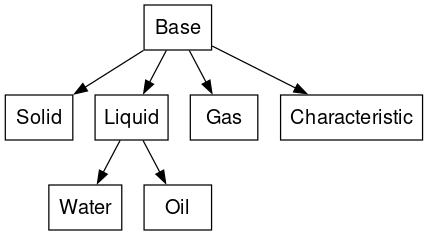
\includegraphics[width=0.45\textwidth]{pictures/test.png}
  \caption{An example of the material hierarchy.}
  \label{fig:MaterialHierarchyExample}
\end{figure}

\subsection{Engineering for Intuition}

\begin{figure}[ht]
  \centering
  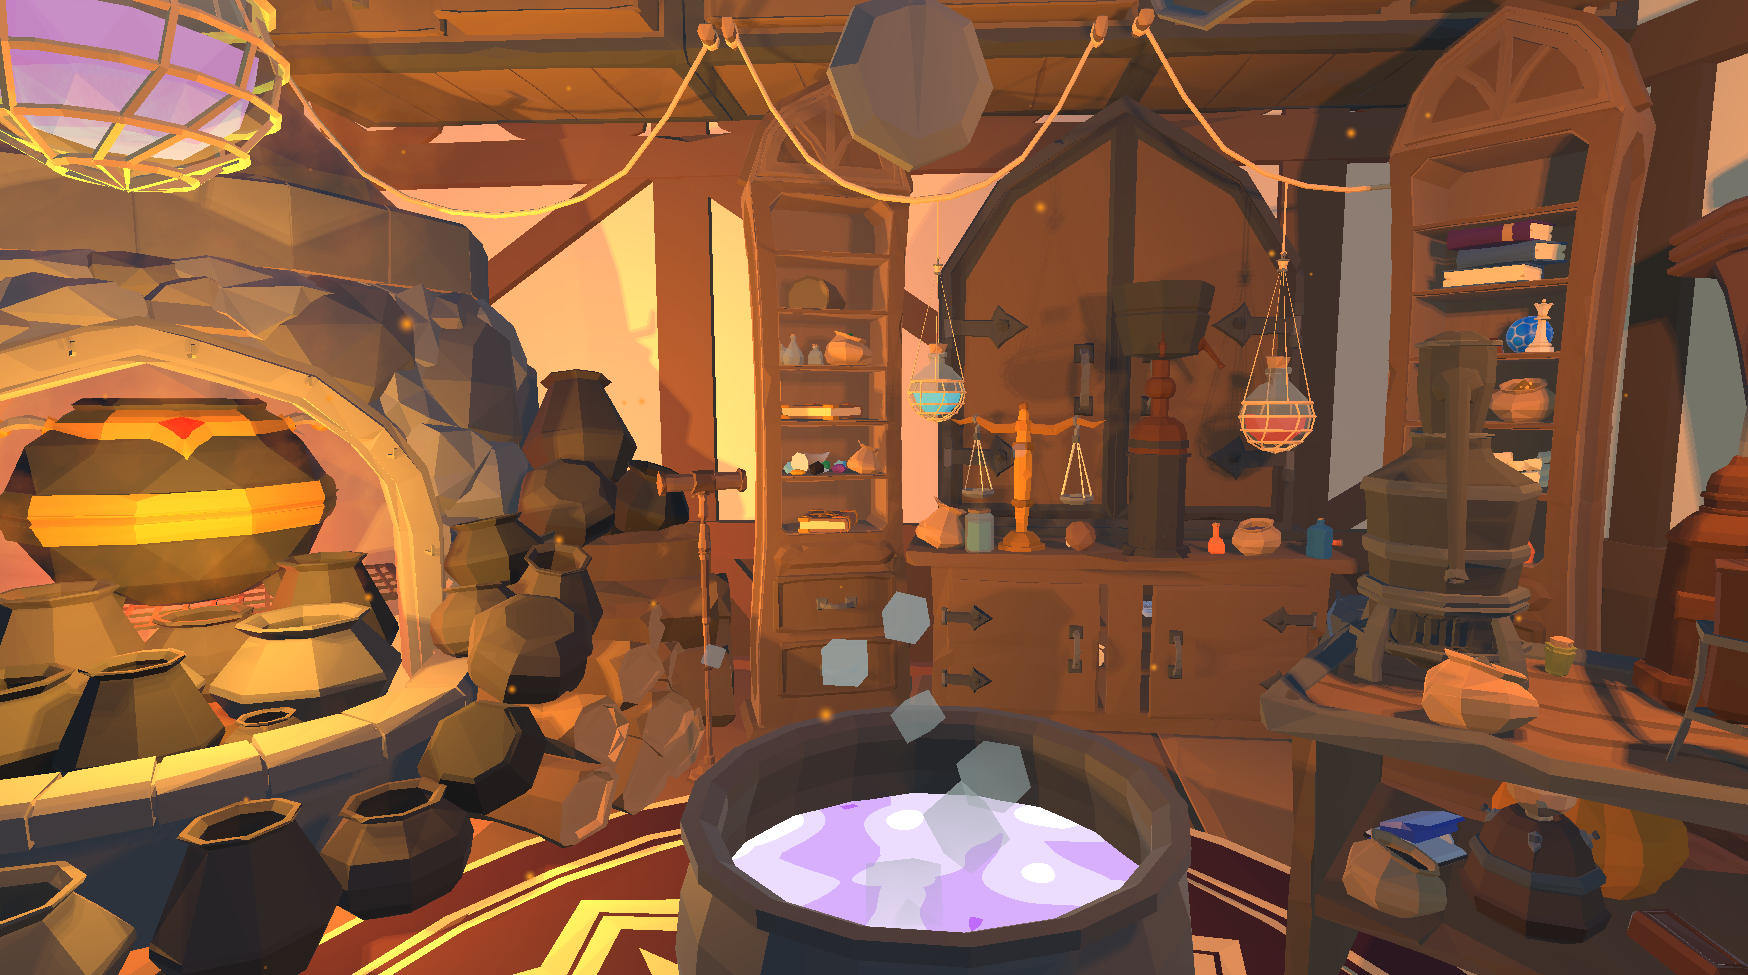
\includegraphics[width=0.45\textwidth]{pictures/Screenshot_1.png}
  \caption{The initial view for the alchemist.}
  \label{fig:InitialView}
\end{figure}

The alchemist is immediately thrown into the game. Instinctively, the first thing they will do is
\textbf{orientate themselves}. This is why the game starts with the alchemist standing in the middle of the room as
seen in figure \ref{fig:InitialView}.

After 5 seconds an \textbf{audible and visual cue} delivers the first task. After communicating with the assistant
a new problem promptly arises for the alchemist: "What are ingredients?".

Intuitively, the alchemist will try to pick up the first thing his brain classifies as "pick-up-able". Because
almost everything in the room is an ingredient this will work.

Having the object in his hand the alchemist will most likely either throw it into the cauldron or come to the next
problem: "How do I know what to throw into the cauldron?".

While working out what materials are needed, the alchemist needs to scout the house for ingredients. This is where
his curiosity will lead him to try and interact with the \textbf{Ingredient Inspect Station}.

\section{Implementation}

States and ingredient materials are implemented as Unity's \texttt{ScriptableObjects}.

To keep track of the materials, states and transitions, they are tracked in a .dot file. By using a simple .dot parser
and some custom editor scripts, the graphs are set up in Unity automatically.

\subsection{Dot Parser}

The .dot parser is kept quite simple and is based mainly on the three regular expressions shown in listing \ref{lst:RegexPatterns}.

\begin{lstlisting}[caption=Regex Patterns, label=lst:RegexPatterns]
  (?:\n *)(\w+)\s*(?:\[(.*?)\])?; //nodes
  (\w+)\s*->\s*(\w+)\s*(?:\[(.*?)\])?; //edges
  (\w+)\s*=\s*(.*?); //attributes
\end{lstlisting}

The parser then returns a simple graph data structure.

\subsection{Ingredient Materials}

Ingredient materials have a name, a parent material and a list of child materials. This allows navigating
the material hierarchy in both directions.

\subsection{Cauldron States}

The cauldron state graph is a directed graph with states as nodes and transitions as edges. Each state holds:

\begin{itemize}
  \item A list of \texttt{CauldronTransitions} that lead to other states
  \item A \texttt{CauldronContentConfig} that holds configuration for the cauldron content shader
  \item A \texttt{CauldronSmokeConfig} that holds configuration for the cauldron smoke particle system
\end{itemize}

These three components are all just \texttt{Serializable} classes as they are not reused anywhere else outside
their state.

\subsection{Cauldron Transitions}

The transitions are defined by a set of required parts (materials and amounts) and a destination state. Using a
simple function that checks if the cauldron contains the required parts, the parent state greedily selects the
first transition that is valid.

\subsection{Cauldron}

The cauldron is in essence just a map of materials to amounts. Whenever an ingredient is thrown into the cauldron
the amount of the materials is increased according to the parts and the material hierarchy. The cauldron also has
a current state that is checked for transitions whenever an ingredient is added.

The cauldron implements the \texttt{IObservable} interface and notifies all observers whenever the state changes.

The cauldron also provides functions that apply \texttt{CauldronContentConfig} and \texttt{CauldronSmokeConfig} to
the shader and particle system.

\subsection{Cauldron Content Shader}

Shader Explanation

\subsection{Ingredients}

Ingredients are \texttt{MonoBehaviour}s that have a name and a list of parts. The script requires a \texttt{Throwable}
component from the SteamVR plugin.

\subsection{Ingredient Inspect Station}

To allow the alchemist to inspect ingredients and their composition the \texttt{IngredientInspectStation} is used.
Using a trigger area the station detects when an ingredient is placed on it. Displaying the ingredient's name and
composition is done via a \texttt{TextMeshPro} component. To animate the text a simple coroutine is used.

\subsection{Audio System}

To make playing audio clips in 3D space easier, a simple audio manager and helper class is used. The audio manager
has a pool of \texttt{AudioSource}s that can be used to play audio clips. The helper class provides a simple interface
to play audio clips at a given position.

\section{Stumbling Blocks}

\subsection{SteamVR Don't Destroy On Load}

The SteamVR player prefab comes standard with the \emph{DontDestroyOnLoad} flag set. Together with default Throwable setting
of not restoring the parent on release, this leads to the duplication of the player and everything he held at some point when
reloaing the scene.

This was fixed by setting the \emph{Do Not Destroy} flag to false in \texttt{Player -> SteamVRObjects -> [SteamVR]}.

\acknowledgments{
  The author wishes to thank Schmidt Alexander, Schachinger Julian and Unterberger Bernhard for testing and
  providing valuable feedback.}

\end{document}